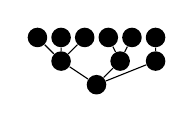
\begin{tikzpicture}[scale=.2]
\node[circle, scale=0.75, fill] (tid0) at (4.5,1.5){};
\node[circle, scale=0.75, fill] (tid1) at (2.25,3){};
\node[circle, scale=0.75, fill] (tid4) at (0.75,4.5){};
\node[circle, scale=0.75, fill] (tid5) at (2.25,4.5){};
\node[circle, scale=0.75, fill] (tid6) at (3.75,4.5){};
\draw[](tid1) -- (tid4);
\draw[](tid1) -- (tid5);
\draw[](tid1) -- (tid6);
\node[circle, scale=0.75, fill] (tid2) at (6,3){};
\node[circle, scale=0.75, fill] (tid7) at (5.25,4.5){};
\node[circle, scale=0.75, fill] (tid8) at (6.75,4.5){};
\draw[](tid2) -- (tid7);
\draw[](tid2) -- (tid8);
\node[circle, scale=0.75, fill] (tid3) at (8.25,3){};
\node[circle, scale=0.75, fill] (tid9) at (8.25,4.5){};
\draw[](tid3) -- (tid9);
\draw[](tid0) -- (tid1);
\draw[](tid0) -- (tid2);
\draw[](tid0) -- (tid3);
\end{tikzpicture}
%%% Local Variables:
%%% TeX-master: "thesis/thesis.tex"
%%% End: 